\chapter{Calculus of Variations}

\section{Directional Derivatives}
\paragraph{Recall:} To minimize $g(u)$, let $u^*$ be a candidate minimizer and pitch a perturbation on $u^*$ of $\varepsilon v$, where $\varepsilon$ is the scale and $v$ is the direction. Taking Taylor's expansion at the perturbation produces

\begin{center}
  \begin{tikzpicture}
    \node [dot] (a) at (0,0) {};
    \node [dot] (b) at (3,1) {};
    \draw [>=latex,->,thick] (a) node [anchor=east] {$u^*$} -- (b) node [anchor=west] {$u^*+\varepsilon v$};
  \end{tikzpicture}
\end{center}

\begin{gather}
  g(u^* + \varepsilon v) = g(u^*) + \varepsilon \pder{g}{u}(u^*) v + o(\varepsilon) \\
  \text{FONC: } \pder{g}{u}(u^*) = 0 \hspace{3cm} 
\end{gather}

\subparagraph{Note:} $\pder{g}{u}(u^*) v$ tells us how much $g(u)$ increases/decreases in the direction of $v$.

\begin{defi}
  The directional (Gateaux) derivative is given by
  \[ \delta g(u;v) = \lim_{\varepsilon\to0} \frac{g(u+\varepsilon v)-g(u)}{\varepsilon} \]
\end{defi}

\paragraph{Example}
\[ g(u) = \frac12 u_1^2 - u_1 + 2u_2, \quad g:\R^2\to\R \]
Let's consider $e_1=[1\ 0]\trans$, $e_2=[0\ 1]\trans$. What is $\delta g(u;e_i)$, $i=1,2$?
\begin{align}
  \delta g(u;v) &= \lim_{\varepsilon\to0} \frac{g(u+\varepsilon v)-g(u)}{\varepsilon} \\
                &= \lim_{\varepsilon\to0} \frac{g(u)+\varepsilon\pder{g}{u}(u) v + o(\varepsilon) - g(u)}{\varepsilon} \\
                &= \pder{g}{u} (u) v
\end{align}
\begin{align}
  \pder{g}{u}(u) &= [u_1-1\ 2] \\
  \delta g(u;e_1) &= [u_1-1\ 2] e_1 = u_1-1 \\
  \delta g(u;e_2) &= [u_1-1\ 2] e_2 = 2 \\
\end{align}

But the beauty of directional derivatives is that they generalize beyond vectors, $u\in\R^m$, to function spaces ($\mathcal U$) or other ``objects'' like matrices.

\paragraph{Example} $M\in\R^{n\times n}$, $F(M)=M^2$

What is $\pder{F}{M}$? (ponder at home\dots)

We can easily compute $\delta F(M;N)$!
\begin{align}
  F(M+\varepsilon N) &= (M+\varepsilon N)(M+\varepsilon N) = M^2 + \varepsilon M N + \varepsilon N M + \varepsilon^2 N^2 \\
  \delta F(M;N) &= \lim_{\varepsilon\to0} \frac{F(M+\varepsilon N)-F(M)}{\varepsilon} \\
                     &= \lim_{\varepsilon\to0} \frac{\varepsilon M N + \varepsilon N M + \varepsilon^2 N^2}{\varepsilon} = MN + NM
\end{align}

\paragraph{Infinite Dimensional Optimization}
Let $u\in\mathcal U$ (function space) and let $J(u)$ be the cost:
\[ \min_{u\in\mathcal U} J(u) \]

\begin{thm}
  If $u^*\in\mathcal U$ is a (local) minimizer then
  \[ \delta J(u^*;v) = 0, \quad \forall v\in\mathcal U \]
\end{thm}

\paragraph{Example} Find minimizer $u^*$ to
\[ J(u) = \int_0^T L(u(t)) \dif t \]
\begin{align}
  J(u+\varepsilon v) - J(u) &= \int_0^T L(u(t)+\varepsilon v(t)) \dif t - \int_0^T L(u(t)) \dif t, \quad u,v\in\mathcal U \\
                            &= \int_0^T \left[ L(u(t)) + \varepsilon \pder{L}{u}(u(t)) v(t) + o(\varepsilon) - L(u(t)) \right] \dif t \\
  \delta J(u^*;v) &= \lim_{\varepsilon\to0} \frac{J(u+\varepsilon v)-J(u)}{\varepsilon} \\
                            &= \lim_{\varepsilon\to0} \frac{\int_0^T \varepsilon \pder{L}{u}(u(t)) v(t) \dif t + o(\varepsilon)}{\varepsilon} \\
                            &= \int_0^T \pder{L}{u}(u(t)) v(t) \dif t \\
\end{align}
$u^*$ optimizer:
\begin{gather}
  \delta J(u^*;v) = \int_0^T \pder{L}{u}(u(t)) v(t) \dif t = 0 \quad \forall v\in\mathcal U \\
  \Updownarrow \\
  \pder{L}{u} (u(t)) = 0 \quad \forall t\in[0,T]
\end{gather}
But, we want \emph{optimal control}! We want our cost to look like
\begin{gather}
  \int_0^T L(x(t),u(t)) \dif t \\
  \dot x = f(x,u)
\end{gather}

\section{Calculus of Variations}
What happens to $x(t)$ when $u(t)$ changes to $u(t)+\varepsilon v(t)$? Let the system be given by
\[ \begin{cases}
    \dot x = f(x,u) \\
    x(0) = x_0
  \end{cases} \]
After perturbation of $u$, the new system is
\[ \begin{cases}
    \dot{\hat x} = f(\hat x,u+\varepsilon v) \\
    x(0) = x_0
  \end{cases} \]

\pgfmathsetseed{11}
\begin{figure}
  \centering
  \begin{tikzpicture}
    \draw [thick,->] (-0.5,0) -- (4,0) node [anchor=west] {$t$};
    \draw [thick,->] (0,-0.5) -- (0,3) node [anchor=east] {};
    \draw [decorate, decoration={random steps, segment length=7pt, amplitude=5pt}, rounded corners=2pt] (0,1) to[in=180,out=0,distance=3.5cm] (3.5,1) node [anchor=south west] {$u(t)$};
    \draw [decorate, decoration={random steps, segment length=8pt, amplitude=5pt}, rounded corners=3pt] (0,2) to[in=180,out=0,distance=3cm] (3.5,2.5) node [anchor=south] {$u(t)+\varepsilon v(t)$};

    \draw [thick,->] (5,0) -- (9.5,0) node [anchor=west] {$t$};
    \draw [thick,->] (5.5,-0.5) -- (5.5,3) node [anchor=east] {};
    \draw [decorate, decoration={random steps, segment length=8pt, amplitude=4pt}, rounded corners=3pt] (5.5,0.75) node [anchor=east] {$x_0$} to[in=200,out=0,distance=3cm] (9,1.5) node [anchor=south west] {$x(t)$};
    \draw [decorate, decoration={random steps, segment length=8pt, amplitude=5pt}, rounded corners=2pt] (5.5,0.75) node [anchor=east] {$x_0$} to[in=170,out=30,distance=3cm] (9,2.5) node [anchor=south,yshift=5pt] {$\hat x(t)=x+\varepsilon\eta+o(\varepsilon),\ \eta(0)=0$};
    \node [dot] at (5.5,0.75) {};
  \end{tikzpicture}
  \caption{Variation in $u$ causes a variation in $x$.}
  \label{fig:var_u_x}
\end{figure}

\noindent
Consider
\[ \tilde x=x+\varepsilon \eta, \]
where
\begin{alignat}{2}
  \dot x&=f(x,u), & x(0) &= x_0 \\
  \dot \eta &= \pder{f}{x}(x,u) \eta + \pder{f}{u}(x,u) v, \qquad & \eta(0) &= 0
\end{alignat}

\begin{thm}
  If $f$ is continuously differentiable in $x$ and $u$ then
  \[ \hat x(t) = \tilde x(t) + o(\varepsilon) \]
  \begin{proof}
    \mbox{}
    \begin{enumerate}[label=\roman*)]
    \item Initial conditions:
      \begin{align}
        \hat x(0) &= x_0 \\
        \tilde x(0) &= x(0) + \varepsilon \eta(0) = x_0
      \end{align}
    \item Dynamics:
      \begin{align}
        \dot{\hat x} &= f(\hat x,u+\varepsilon v) \\
        \dot{\tilde x} &= \dot x + \varepsilon \dot \eta = f(x,u) + \varepsilon \pder{f}{x}(x,u)\eta + \varepsilon \pder{f}{u}(x,u) v \\
                     &= f(x+\varepsilon\eta,u+\varepsilon v) + o(\varepsilon) \\
                     &= f(\tilde x,u+\varepsilon v) + o(\varepsilon)
      \end{align}
      We can see that the dynamics of $\hat x(t)$ are equal to those of $\tilde x(t)$ plus higher order terms:
      \begin{align}
        \dot{\tilde x} &= f(\tilde x,u+\varepsilon v) + o(\varepsilon) \\
        \dot{\hat x} &= f(\hat x,u+\varepsilon v)
      \end{align}
      Therefore, if our perturbation is small enough, we can model $\hat x(t)$ as $\tilde x(t)$.
    \end{enumerate}
  \end{proof}
\end{thm}

\begin{framed}
  \hypertarget{taylor_2var}{}
  Note: Taylor expansion with two elements is
  \begin{align}
    h(w+\varepsilon v,z+\varepsilon y) &= h(w,z+\varepsilon y) + \pder{h}{w}(w,z+\varepsilon y)\varepsilon v + o(\varepsilon) \\
                                       &= \left\{ h(w,z) + \pder{h}{z}(w,z)\varepsilon y + o(\varepsilon) \right\} \\
                                       & \qquad + \left\{ \pder{h}{w}(w,z)\varepsilon v + \underbrace{\pder{^2 h}{z\partial w}\varepsilon v \odot \varepsilon y}_{o(\varepsilon)} + o(\varepsilon) \right\} \\
                                       &= h(w,z) + \pder{h}{z}\varepsilon y + \pder{h}{w}\varepsilon v + o(\varepsilon)
  \end{align}
\end{framed}

% 2017/01/26
\paragraph{Last class:} \mbox{}
\begin{enumerate}
\item $u\in\U$ (space of functions), $J:\U\to\R$ (cost).

  FONC: If $u^*$ is optimal, then
  \[ \delta J(u;\nu) = 0 \quad \forall \nu\in\U, \]
  where the directional derivative is given by
  \[ \delta J(u;\nu) = \lim_{\varepsilon\to0} \frac{J(u+\varepsilon \nu)-J(u)}{\varepsilon}. \]
\item If
  \[ \begin{cases}
      \dot x = f(x,u) \\
      x(0) = x_0
    \end{cases} \]
  then a variation in $u$:
  \[ u \longmapsto u+\varepsilon \nu \]
  results in a variation in $x$:
  \[ x \longmapsto x+\varepsilon\eta + o(\varepsilon) \]
  See \autoref{fig:var_u_x}. Note $\eta(0)=0$.
\end{enumerate}

\subsection{An (Almost) Optimal Control Problem}

Let $\dot x=f(x)$, $x(0)=x_0$. Note we get to pick the initial condition!
\subparagraph{Problem}
\begin{gather}
  \min_{x_0\in\R^m} J(x_0) = \int_0^T L(x(t)) \dif t \\
  \text{s.t. } \begin{cases}
    \dot x(t) = f(x(t)) & \text{the \emph{constraint}! (equality)} \\
    x(0)=x_0
  \end{cases}
\end{gather}
Note every constraint needs a Lagrange multiplier. We have infinitely many constraints:
\[ \dot x(t) = f(x(t)) \quad \forall t\in[0,T] \]
We need $\lambda(t)$ as a function of $t$. Also, the sum in the Lagrangian has to become an integral. The continuous-time Lagrangian thus becomes
\[ \tilde J(x_0,\lambda) = \int_0^T \Big[ L(x(t)) + \lambda\trans(t) (f(x(t))-\dot x(t)) \Big] \dif t \]
The task is to perturb $x_0$ as $x_0\longmapsto x_0+\varepsilon \nu$, $\nu\in\R^m$ and compute
\[ \delta \tilde J(x_0;\nu) = \lim_{\varepsilon\to0} \frac{\tilde J(x_0+\varepsilon \nu)-\tilde J(x_0)}{\varepsilon} \]
and make this equal to 0 $\forall \nu\in\R^m$. The variation in $x$ is

\pgfmathsetseed{11}
\begin{center}
  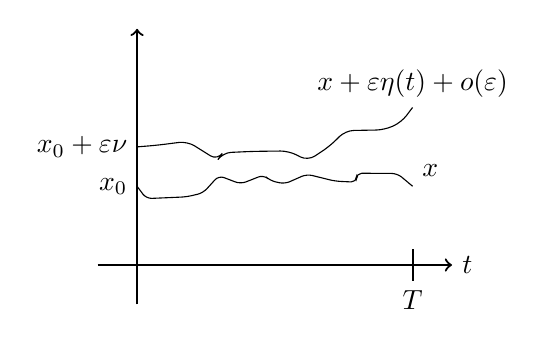
\begin{tikzpicture}
    \draw [->,thick] (-0.5,0) -- (4,0) node [anchor=west] {$t$};
    \draw [->,thick] (0,-0.5) -- (0,3);
    \draw [decorate, decoration={random steps, segment length=7pt, amplitude=5pt}, rounded corners=2pt] (0,1) node [anchor=east] {$x_0$} to[in=180,out=0,distance=3.5cm] (3.5,1) node [anchor=south west] {$x$};
    \draw [decorate, decoration={random steps, segment length=9pt, amplitude=5pt}, rounded corners=3pt] (0,1.5) node [anchor=east] {$x_0+\varepsilon \nu$} to[in=200,out=0,distance=3.5cm] (3.5,2) node [anchor=south] {$x+\varepsilon\eta(t)+o(\varepsilon)$};
    \draw [thick] (3.5,0.2) -- (3.5,-0.2) node [anchor=north] {$T$};
  \end{tikzpicture}
\end{center}

Note:

\hspace{\parindent}
\begin{tabular}{cl}
  $x_0$ & decision variable \\
  $\nu$ & variation in $x_0$ \\
  $x(t)$ & trajectory starting at $x_0$ \\
  $\eta(t)$ & change in trajectory resulting from $\nu$-variation in $x_0$ \\
  $\lambda(t)$ & time-varying Lagrange multiplier
\end{tabular}

\begin{align}
  \tilde J(x_0+\varepsilon \nu) &= \int_0^T \Big\{ L(x(t)) + \lambda\trans(t) [f(x(t)+\varepsilon\eta(t)) - \dot x(t) - \varepsilon\dot\eta(t)] \Big\} \dif t + o(\varepsilon) \\
                                &= \int_0^T \left[ L(x) + \varepsilon\pder{L}{x}(x)\eta + \lambda\trans \left( f(x) + \varepsilon\pder{f}{x}(x)\eta - \dot x - \varepsilon\dot\eta \right) \right] \dif t + o(\varepsilon) \\
  \tilde J(x_0+\varepsilon \nu) - \tilde J(x_0) &= \int_0^T \left[ \varepsilon\pder{L}{x}(x)\eta + \lambda\trans\left( \varepsilon\pder{f}{x}\eta - \varepsilon\dot\eta \right) \right] \dif t + o(\varepsilon) \\
  \delta \tilde J (x_0;\nu) &= \int_0^T \left[ \pder{L}{x}(x)\eta + \lambda\trans\left( \pder{f}{x}\eta - \dot\eta \right) \right] \dif t
\end{align}
A powerful idea: we want $\delta\tilde J(x_0;\nu)=0$ $\forall \nu$. Somehow get this in the form
\[ \int_0^T \Big(\text{stuff}(t)\Big) \eta(t) \dif t = 0 \]
We can pick $\text{stuff}(t)=0$ $\forall t\in[0,T]$.

In $\delta\tilde J(x_0;\nu)$ we have $\dot\eta$ (problem!). We can solve this using \emph{integration by parts}.
\[ \int_0^T \lambda\trans \dot\eta \dif t = \lambda\trans(T)\eta(T) - \lambda\trans(0)\eta(0) - \int_0^T \dot\lambda\trans\eta \dif t \]
Hence,
\[
  \delta\tilde J(x_0;\nu) = \int_0^T \underbrace{\big( \pder{L}{x} + \lambda\trans\pder{f}{x} + \dot\lambda\trans \big)}_{\text{pick}=0} \eta \dif t - \underbrace{\lambda\trans(T)}_{\text{pick}=0} \eta(T) + \lambda\trans(0) \underbrace{\eta(0)}_{\nu}
\]
We are free to pick $\lambda$ freely if it gives $\delta\tilde J=0$.
\[ \text{Pick: } \begin{cases}
    \dot\lambda(t) = -\pder{L\trans}{x}(x(t)) - \pder{f\trans}{x}(x(t)) \lambda(t) \\
    \lambda(T) = 0 & \text{backwards diff. eq}
  \end{cases} \]
Under this choice of $\lambda$ we get
\[ \delta\tilde J(x_0;\nu) = \lambda\trans(0) \nu \]
This is linear in $\nu$ so the FONC is $\lambda(0)=0$.

Moreover, we really have a ``normal'' optimization problem
\begin{gather}
  \min_{x_0\in\R^m} \tilde J(x_0) \\
  \delta \tilde J(x_0;\nu) = \pder{\tilde J}{x_0} (x_0) \nu
\end{gather}
which means that
\[ \pder{\tilde J}{x_0} = \lambda\trans(0) \]
If $x_0^*$ minimizes
\begin{gather}
  \int_0^T L(x(t)) \dif t \\
  \text{s.t. } \begin{cases}
    \dot x(t) = f(x(t)) \\
    x(0) = x_0^*
  \end{cases}
\end{gather}
then
\[ \lambda(0) = \bm 0 \]
where $\lambda(t)$ satisfies
\[ \begin{cases}
    \dot \lambda(t) = -\pder{L\trans}{x}(x(t)) - \pder{f\trans}{x}(x(t)) \lambda(t) \\
    \lambda(T) = 0
  \end{cases} \]

\paragraph{So what?} We actually have a two-point boundary value problem. 
\begin{align}
  \dot x &= f(x) & \dot\lambda &= -\pder{L\trans}{x} - \pder{f\trans}{x} \lambda \\
  x(0) &= x_0 & \lambda(T) &= 0
\end{align}

\begin{center}
  \begin{tikzpicture}
    \draw [thick,->] (0,0) -- (4,0) node [anchor=west] {$t$};
    \draw [thick,->] (0,0) -- (0,3);
    \draw (-0.2,1.5) node [anchor=east] {$x_0$} -- (0.2,1.5);
    \draw [->,>={Straight Barb[scale length=2]}] (0,1.5) parabola bend (0.6,2) (1.5,1.5);
    \draw (1.5,1.5) parabola bend (2,1.3) (3.5,2.5);

    \draw [thick,->] (6,0) -- (10,0) node [anchor=west] {$t$};
    \draw [thick,->] (6,0) -- (6,3);
    \draw (9.5,0.2) -- (9.5,-0.2) node [anchor=north] {$T$};
    \draw [-{Straight Barb[scale length=2]}] (9.5,0) .. controls (8.25,0) and (9,1.5) .. (8,1.5) node [anchor=south] {$\lambda$};
    \draw (8,1.5) .. controls (7,1.25) .. (6,1.5);
    \draw (6.2,1.5) -- (5.8,1.5) node [anchor=east] {$\lambda(0)$};
  \end{tikzpicture}
\end{center}
We want to find $x_0$ that gives $f(x)$ such that after solving backwards for $\lambda(t)$, we find that
\[ \lambda(0) = \pder{\tilde J\trans}{x_0} = 0. \]
This leads to the following:

\paragraph{An algorithm} \mbox{}

\begin{algorithm}
  \begin{algorithmic}
    \State Pick $x_{0,0}$
    \State $k=1$
    \Repeat
    \State Simulate $x(t)$ from $x_{0,k}$ over $[0,T]$
    \State Simulate $\lambda(t)$ from $\lambda(T)=0$ backwards using $x(t)$
    \State Update $x_{0,k}$ as
    $ x_{0,k+1} = x_{0,k} - \gamma\lambda(0) $ \Comment{$\lambda(0)$ is the gradient}
    \State $k\coloneqq k+1$
    \Until $\lambda(0)=0$
  \end{algorithmic}
\end{algorithm}

\paragraph{Example:} \texttt{optinit.m}

\[ \dot x = Ax, \quad L=x\trans Qx-q, \quad Q=Q\trans \succ 0 \]
\vspace{-2em}
\begin{align}
  \dot \lambda &= -2Qx - A\trans\lambda \\
  \lambda(0) &= 0
\end{align}

% 2017/01/31
\subsection{Optimal Timing Control}
When to switch between modes?
\begin{equation}
  \begin{aligned}
    \dot x &= \begin{cases}
      f_1(x) & \text{if } t\in[0,\tau) \\
      f_2(x) & \text{if } t\in[\tau,T]
    \end{cases} \\
    x(0) &= x_0
  \end{aligned} \label{eq:otc}
\end{equation}

\begin{center}
  \begin{tikzpicture}
    \draw [->,thick] (-0.2,0) -- (5.5,0) node [anchor=west] {$t$};
    \draw [->,thick] (0,-0.2) -- (0,3.2);
    \draw (4.8,0.2) -- (4.8,-0.2) node [anchor=north] {$T$};
    \draw (2.2,0.2) -- (2.2,-0.2) node [anchor=north] {$\tau$};
    \draw (0.2,1) -- (-0.2,1) node [anchor=east] {$x_0$};
    \draw (0,1) parabola (2.2,2.8);
    \draw (2.2,2.8) parabola [bend at end] (4.8,1.2) node [anchor=west] {$x$};
    \node at (1,1.8) {$f_1$};
    \node at (4,1.8) {$f_2$};
  \end{tikzpicture}
\end{center}

\begin{align}
  & \min_\tau \int_0^T L(x(t)) \dif t = J(\tau) \\
  & \text{s.t.~\eqref{eq:otc} holds}
\end{align}

\begin{enumerate}[label=Step \arabic*:]
\item Augment cost with constraint
  \[ \tilde J = \int_0^\tau \Big[ L(x) + \lambda\trans(f_1(x)-\dot x) \Big] \dif t + \int_\tau^T \Big[ L(x) + \lambda\trans(f_2(x)-\dot x) \Big] \dif t \]
\item Variation $\tau\longmapsto\tau+\varepsilon\theta$
  \begin{center}
    \begin{tikzpicture}
      \draw [->,thick] (-0.2,0) -- (5.5,0) node [anchor=west] {$t$};
      \draw [->,thick] (0,-0.2) -- (0,3.2);
      \draw (4.8,0.2) -- (4.8,-0.2) node [anchor=north] {$T$};
      \draw (2.2,0.2) -- (2.2,-0.2) node [anchor=north] {$\tau$};
      \draw (3,0.2) -- (3,-0.2) node [anchor=north,yshift=3pt] {$\tau+\varepsilon\theta$};
      \draw (0.2,1) -- (-0.2,1) node [anchor=east] {$x_0$};
      \draw (0,1) parabola (2.2,1.8);
      \draw (2.2,1.8) parabola [bend at end] (4.8,1.2) node [anchor=west] {$x$};
      \node at (1,1.8) {$f_1$};
      \node at (3.6,1.7) {$f_2$};

      \begin{scope}
        \clip (4.8,4) rectangle (2.2,1.8);
        \draw [dashed] (2.2,1.8) parabola bend (0,1) (3,2.5);
        \draw [dashed] (3,2.5) parabola [bend at end] (5.4,1.9);
      \end{scope}
      \node [anchor=west] at (4.8,1.9) {$x+\varepsilon\eta+o(\varepsilon)$};
      \node at (2.4,2.4) {$f_1$};
      \node at (3.9,2.5) {$f_2$};
    \end{tikzpicture}
  \end{center}
\item Compute $\delta\tilde J(\tau;\theta)$
\end{enumerate}
\begin{align}
  \tilde J(\tau+\varepsilon\theta) &= \int_0^{\tau+\varepsilon\theta} \Big\{ L(x+\varepsilon\eta) + \lambda\trans[f_1(x+\varepsilon\eta)-\dot x-\varepsilon\dot\eta] \Big\} \dif t \\
                                   & \qquad + \int_{\tau+\varepsilon\theta}^T \Big\{ L(x+\varepsilon\eta) + \lambda\trans[f_2(x+\varepsilon\eta)-\dot x-\varepsilon\dot\eta] \Big\} \dif t + o(\varepsilon) \\
  \intertext{Note that $\eta=\dot\eta=0$ on $[0,\tau)$.}
  \tilde J(\tau+\varepsilon\theta) &= \int_0^\tau \Big\{ L(x) + \lambda\trans[f_1(x)-\dot x] \Big\} \dif t \\
                                   & \qquad + \int_\tau^{\tau+\varepsilon\theta} \Big\{ \underbrace{L(x+\varepsilon\eta)}_{L(x)+\varepsilon\pder{L}{x}\eta} + \lambda\trans[\underbrace{f_1(x+\varepsilon\eta)}_{f_1(x)+\varepsilon\pder{f_1}{x}\eta} - \dot x-\varepsilon\dot\eta] \Big\} \dif t \\
                                   & \qquad + \int_{\tau+\varepsilon\theta}^T \Big\{ \underbrace{L(x+\varepsilon\eta)}_{L(x)+\varepsilon\pder{L}{x}\eta} + \lambda\trans[\underbrace{f_2(x+\varepsilon\eta)}_{f_2(x)+\varepsilon\pder{f_2}{x}\eta} - \dot x-\varepsilon\dot\eta] \Big\} \dif t + o(\varepsilon) \displaybreak \\
  \delta\tilde J(\tau;\theta) &= \lim_{\varepsilon\to0} \frac{\tilde J(\tau+\varepsilon\theta) - \tilde J(\tau)}{\varepsilon} \\
  \tilde J(\tau+\varepsilon\theta) - \tilde J(\tau) &= \int_0^\tau 0\cdot\dif t + \underbrace{ \int_\tau^{\tau+\varepsilon\theta} \left[ \varepsilon\pder{L}{x}\eta + \lambda\trans \Big(f_1(x)+\varepsilon\pder{f_1}{x}\eta - f_2(x) - \varepsilon\dot\eta \Big) \right] \dif t }_{\displaystyle I_1} \\
                                   & \qquad + \underbrace{ \int_{\tau+\varepsilon\theta}^T \left[ \varepsilon\pder{L}{x}\eta + \lambda\trans \Big( \varepsilon\pder{f_2}{x}\eta - \varepsilon\dot\eta \Big) \right] \dif t }_{\displaystyle I_2} + o(\varepsilon)
\end{align}

\begin{framed}
  \begin{thm}[Mean-value theorem]
    \[ \int_{t_1}^{t_2} h(t) \dif t = (t_2-t_1) h(\xi) \quad \text{for some}\ \xi\in[t_1,t_2] \]
  \end{thm}
\end{framed}

\noindent
The first integral is
\begin{align}
  I_1 &= \int_\tau^{\tau+\varepsilon\theta} \left\{ \varepsilon\pder{L}{x}\eta + \lambda\trans \left[f_1(x)+\varepsilon\pder{f_1}{x}\eta-\varepsilon\dot\eta-f_2(x)\right] \right\} \dif t \\
      &= \varepsilon\theta \Big\{ \lambda\trans(\xi) \big[ f_1(x(\xi)) - f_2(x(\xi)) \big] \Big\} + o(\varepsilon)
\end{align}
Note that as $\varepsilon\to0$, $\xi\to\tau$. Using integration by parts, the second integral is
\begin{align}
  \int_\tau^T \lambda\trans \dot\eta \dif t &= \lambda\trans(T) \eta(T) - \lambda\trans(\tau) \underbrace{\eta(\tau)}_{=0} - \int_\tau^T \dot\lambda\trans \eta \dif t \\
  I_2 &= \int_\tau^T \left[ \varepsilon\pder{L}{x}\eta + \lambda\trans \Big( \varepsilon\pder{f_2}{x}\eta - \varepsilon\dot\eta \Big) \right] \dif t - \underbrace{ \int_\tau^{\tau+\varepsilon\theta} \left[ \varepsilon\pder{L}{x}\eta + \lambda\trans \Big( \varepsilon\pder{f_2}{x}\eta - \varepsilon\dot\eta \Big) \right] \dif t }_{o(\varepsilon)} \\
                                            &= \varepsilon \int_\tau^T \left[ \pder{L}{x} + \lambda\trans \pder{f_2}{x} + \dot\lambda\trans \right] \eta \dif t - \varepsilon \lambda\trans(T)\eta(T) + o(\varepsilon)
\end{align}
Hence,
\begin{align}
  \delta\tilde J(\tau;\theta) &= \lim_{\varepsilon\to0} \frac{\tilde J(\tau+\varepsilon\theta) - \tilde J(\tau)}{\varepsilon} \\
                              &= \theta\lambda\trans(\tau) \Big[ f_1(x(\tau)) - f_2(x(\tau)) \Big] + \int_\tau^T \left[ \pder{L}{x} + \lambda\trans \pder{f_2}{x} + \dot\lambda\trans \right] \eta \dif t - \lambda\trans(T)\eta(T)
\end{align}

\begin{enumerate}[resume*]
\item Select the \emph{costate} $\lambda(t)$. The key idea is to get rid of any term that has $\eta$ in it, i.e.
  \begin{align}
    \dot\lambda &= -\pder{L\trans}{x} - \pder{f_2\trans}{x} \lambda \quad \text{on } [\tau,T] \\
    \lambda(T) &= 0
  \end{align}
\item With this choice of $\lambda(t)$, we have
  \[ \delta\tilde J(\tau;\theta) = \theta\lambda\trans(\tau) \Big[ f_1(x(\tau)) - f_2(x(\tau)) \Big] = \pder{\tilde J}{\tau} \theta. \]
  Therefore,
  \[ \pder{\tilde J}{\tau} = \lambda\trans(\tau) \Big[ f_1(x(\tau)) - f_2(x(\tau)) \Big] = 0 \quad \text{(for optimality)} \]
\end{enumerate}

\paragraph{Algorithm} \mbox{}
\begin{algorithm}
  \begin{algorithmic}
    \State Pick $\tau_0$
    \State $k=0$
    \Repeat
    \State Simulate $x$ forward in time from $x(0)=x_0$
    \State Simulate $\lambda$ backwards from $\lambda(T)=0$
    \State Update $\tau_k$ as
    $ \tau_{k+1} = \tau_k - \gamma\lambda\trans(\tau_k) \big[ f_1(x(\tau_k)) - f_2(x(\tau_k)) \big] $
    \State $k\coloneqq k+1$
    \Until $\Vert \lambda\trans(f_1-f_2) \Vert < \varepsilon$
  \end{algorithmic}
\end{algorithm}

Where are we going? Come up with general principles for $\min_{u\in\mathcal U} J(u)$:
\begin{itemize}
\item Costate equations
\item Optimality conditions
\item Algorithms
\item Applications
\end{itemize}

%%% Local Variables:
%%% mode: latex
%%% TeX-master: "../notes"
%%% End:
